\documentclass[12pt]{article}% uses letterpaper by default

%---------- Uncomment one of them ------------------------------
\usepackage[includeheadfoot, top=1in, bottom=1in, hmargin=1in]{geometry}

% \usepackage[a5paper, landscape, twocolumn, twoside,
%    left=2cm, hmarginratio=2:1, includemp, marginparwidth=43pt, 
%    bottom=1cm, foot=.7cm, includefoot, textheight=11cm, heightrounded,
%    columnsep=1cm, dvips,  verbose]{geometry}
%---------------------------------------------------------------
\usepackage{fancyhdr}
\renewcommand{\footrulewidth}{0.4pt}% default is 0pt
\usepackage{verbatim}
\usepackage{url}
\usepackage{cancel}
\pagestyle{fancy}
\usepackage{graphicx}
\usepackage{setspace}
\singlespacing
%\doublespacing
%\onehalfspacing
%\newcommand{\exercisename}{}
\usepackage{varwidth}

\newcommand{\degrees}{\ensuremath{^\circ}}
\newcommand{\arcmin}{\ensuremath{'}}
\newcommand{\arcsec}{\ensuremath{"}}
\newcommand{\hours}{\ensuremath{^\mathrm{h}}}
\newcommand{\minutes}{\ensuremath{^\mathrm{m}}}
\newcommand{\seconds}{\ensuremath{^\mathrm{s}}}

\newcommand{\s}[0]{\phantom{i}} %sets up \s command
\newcommand{\m}[0]{\phantom{abcde}} %sets up \m command
\providecommand{\e}[1]{\ensuremath{\times 10^{#1}}} %sets up \e command
\setlength{\parindent}{0.2in} %new paragraph indent
\usepackage{indentfirst} % indent the first paragraph of a section
\usepackage{amsmath}
\usepackage{enumitem}

\lhead{Astronomy Lab}
\rhead{Observing Lab}
\lfoot{Yahalomi}
\rfoot{Spring 2022}
\cfoot{\thepage}


\begin{document}

\begin{center}
    \LARGE The Moon
\end{center}

\section{Introduction}
In this lab you will learn about the Moon. 
The Moon is the brightest object in the night sky and has played an important role in many cultures throughout the history of mankind. 
It is Earth's only natural satellite and the only extraterrestrial body ever visited by the human beings (but not for much longer, fingers crossed).
In this lab we will investigate the moon in some detail. 
We'll learn about the Moon's orbit and phases, look into why we only see the near side of the Moon, and discover what causes the tides in the oceans. 
We'll also go up onto the roof, and take some measurements and pictures! 


\section{The Moon's Orbit}

\subsection{The Far Side of the Moon}
Over time, tidal forces from the Earth have slowed the Moon's rotation, such that the same side of the Moon always faces the Earth. This causes there to be one side of the Moon that we can see from the Earth and another that we cannot.
The far side of the Moon, sometimes called the ``dark side of the Moon'', is the lunar hemisphere that permanently faces away from the Earth. 
It is therefore not visible from the Earth's surface. 
The far hemisphere was first photographed by the Soviet Luna 3 probe in 1959, and was first directly observed by human eyes when the Apollo 8 mission orbited the Moon in 1968.
Some conspiracy theorists have alleged that some Apollo astronauts had seen UFOs on the far side of the Moon but were told to keep quiet about them. 
Let's figure out why we can't see this mysterious side of the Moon.
\begin{enumerate}
    \item In groups of 3 or 4, assign one person to be the Moon, one person to be the Earth, and one (or two) people to be observers. 
    Have the Moon revolve around the Earth, while always facing it. 
    Have the observers stand outside of the orbit and observe the Moon from a fixed direction. 
    \item The Earth in this scenario will always see the same side of the Moon, by construction. 
    Observers: is that true for you as well?
    If not, what portion of the orbit must the Moon complete before you see the same side again? 
    \item Why do we always see the same side of the Moon? 
    Think about how long it takes for the the moon to complete one orbit around the Earth and how long it takes for the moon to rotate once about its axis. 
    \item Why does the far side of the Moon have more craters?
    \item Why might calling the far side of the Moon the ``dark side'' be confusing?
\end{enumerate}


\subsection{The Moon's Phases}

So we now know that the same side of the moon always faces Earth. This fact, plus the fact that the Moon itself doesn't emit light, but instead is only reflecting light from the Sun, gives us enough information to understand why the Moon appears as it does in the night sky. Over the course of 28 days, the Moon goes through one lunar cycle. A lunar phase is the shape of the sunlit part of the Moon, as seen from Earth. The stages of the Lunar cycle are often divided into eight steps:
\begin{itemize}
    \item New Moon: the Moon isn't visible.
    
    \item Waxing Crescent: A quarter of the ``light side'' of the Moon is visible.
    
    \item First Quarter: Half of the ``light side'' of the Moon is visible.
    
    \item Waxing Gibbous: three quarters of the ``light side'' of the Moon is visible.
    
    \item Full Moon: the full ``light side'' of the Moon is visible.
    
    \item Waning Gibbous: three quarters of the ``light side'' of the Moon is visible.
    
    \item Third Quarter: Half of the ``light side'' of the Moon is visible.
    
    \item Waning Crescent: A quarter of the ``light side'' of the Moon is visible.
\end{itemize}

\begin{figure}[t]
\center
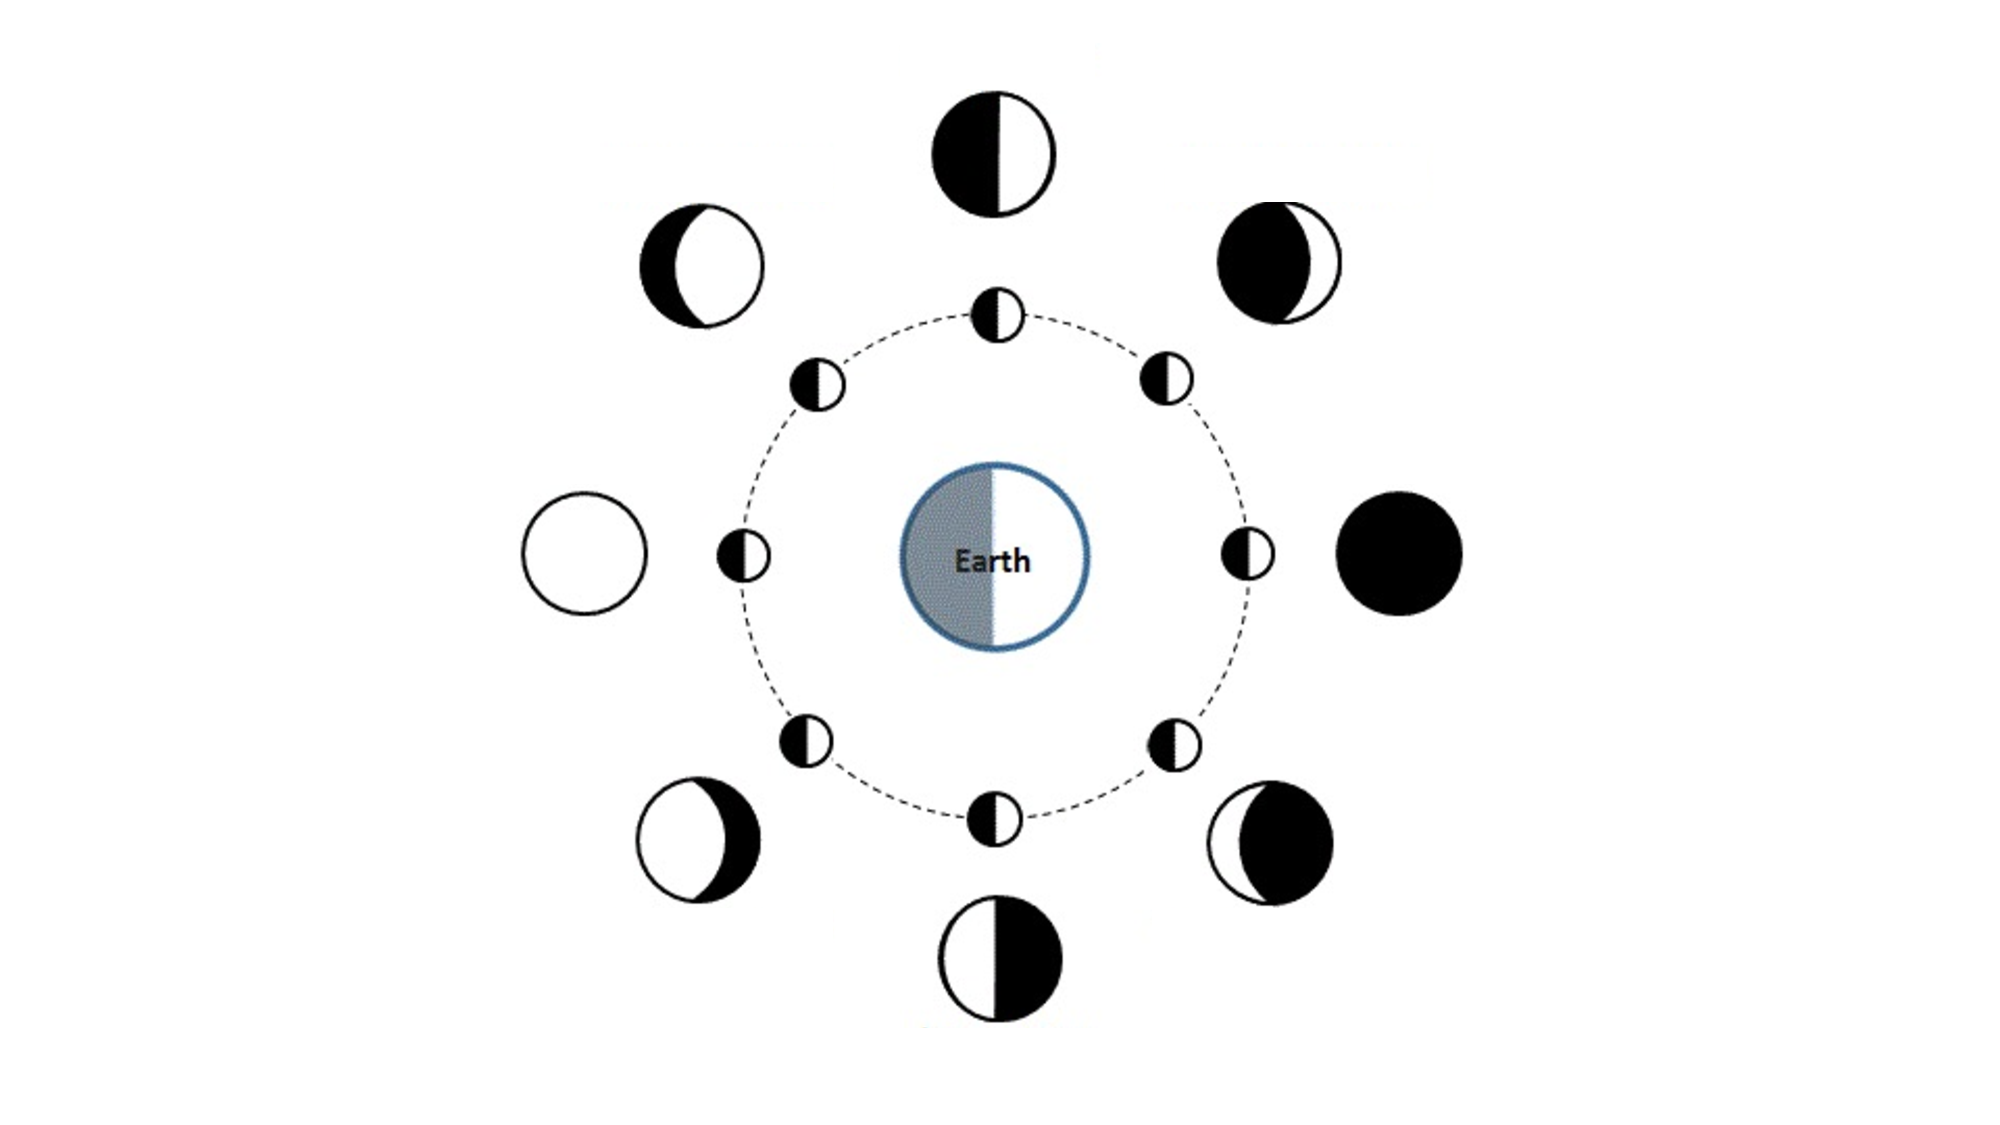
\includegraphics[width=15cm]{lunar_phases.pdf}
\end{figure}

In the figure below, we can see the Earth, and the Moon in these eight phases of its orbit. On the diagram, the 16 smaller circles are the Moon at various phases. The white space in these circles shows the light part of the Moon and the dark space shows the dark parts of the Moon. The smaller Moons (closer to the Earth in the diagram) show the total light reflected by the Moon over time, while the outer circle shows the phase of the Moon, as seen by Earth, over time. 




\begin{enumerate}
\item In the figure, where would you place the Sun? Said differently, where is the sunlight coming from? (Hint: left, right, top or bottom) Why?

\item Can you recognize the phases of the Moon? Which configuration gives a Full Moon? Which gives a New Moon (when you cannot see the moon)? 

\item The orbital period of the Moon is 28 days. If day 1 is the New Moon, then what day is the First Quarter, Full Moon, and Third Quarter?

\end{enumerate}



\subsection{Eclipses}
Now that you are familiar with the motion of the Moon, think about eclipses.
\begin{enumerate}

    \item What is the phase of the Moon during a solar eclipse? During a lunar eclipse?
    
    \item Based on this simplified picture, how often should solar and/or lunar eclipses happen? Is this actually the case? Why or why not?
    
    [Hint: the moon's orbit is inclined by about $5^{\circ}$ to the Earth-Sun plane].
    
\end{enumerate}


\pagebreak
\subsection{Tides}


\begin{figure}[htb!]
\center
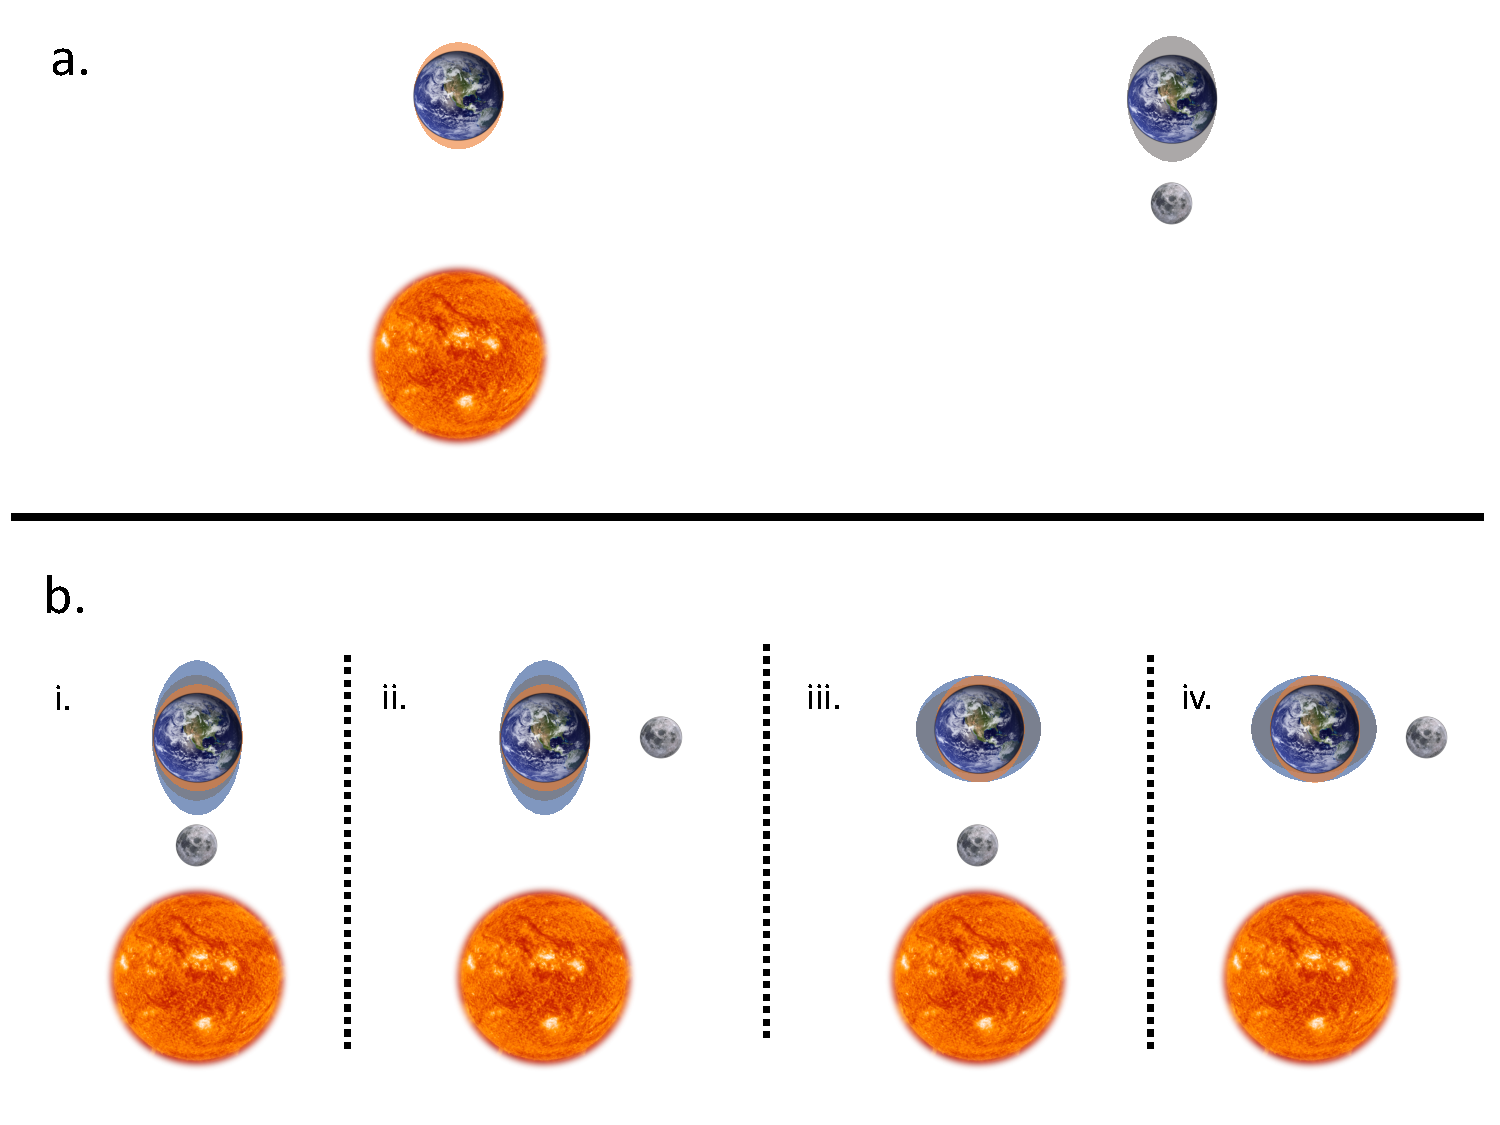
\includegraphics[width=15cm]{tides_fig.pdf}
\end{figure}


Both the Sun and the Moon exert gravitational force to the Earth. 
The Sun is more massive, but the Moon is much closer. Tides in the oceans on Earth are caused by the difference in the gravitational force based on the location of the Sun and the Moon relative to Earth. The moon has a larger effect on the tides of the ocean because it is so much closer to the Earth and so there is a more significant change in gravity on the Oceans based on where the Moon is in its orbit. While the Sun's gravitational pull is larger than the Moon's in total, because it is further, the difference between the Sun's pull on the part of Earth facing it and the part of Earth not facing it is less significant than that of the Moon. The figure above shows the effects of the Sun and the Moon on the ocean tides on Earth. On the top half of the figure (part a.), we can see the effect of the Sun and the Moon independently, the Sun's pull on the tides is shown in orange shading around the Earth on the left and the Moon's shading shown in grey shading around the Earth on the right. On the bottom half of the figure (part b.) we can see 4 configurations of the Earth, Moon, and Sun system: i, ii, iii, and iv. (Hint: 2 of these configurations are physically possible and 2 are not physically possible.)

\begin{enumerate}
    \item High tide, as the name suggests is when the ocean's height or depth increases. Low tide, similarly, is when the the ocean's height or depth decreases. Based on these figures, describe the 2 locations of the Moon (relative to a location on Earth) when we expect high tide and the 2 locations of the Moon (relative to a location on Earth) when we expect low tide. Feel free to draw a diagram if helpful.

    \item In reality, the Sun and the Moon both effect the Ocean tides. Let's combine the Sun's and the Moon's effects on Earth's tides. Based on part a of the figure and your understanding of tides, which two of these four configurations in part b. make physical sense? Why?
    
    \item Which of these four configurations would we expect to cause the highest high tide and the lowest low tide (depending on your location on Earth)? 
    
    \item Which of these four configurations would we expect to cause the lowest high tide and the highest low tide (depending on your location on Earth)? 
\end{enumerate}


\section{Observing the Moon}
We will now observe the Moon with a telescope!

\subsection*{Before we go outside...}
\noindent Draw two large circles on two separate pages in your notebook.
Make sure there is room around the circle for describing and identifying features on the surface.

\subsection*{Once outside...}
\begin{itemize}
    \item How many degrees across is the moon? 
    Make a first order estimate of how many degrees across is the full Moon? In order to do so, we can extend our arm to full length and the width of our pinky finger is about 1$^{\circ}$ across. You may need to measure the degrees across for the portion of the Moon you can see, and then extrapolate to the Full Moon.
    \item Note the time.
    \item Sketch the entire Moon in one of your circles. Note if you can see any specific craters or other features on the Moon.
\end{itemize}

\subsection*{Using the telescope...}
\begin{itemize}
    \item Sketch one section of the Moon, i.e. a ``close up''. 
    Use the telescope in the large dome to help with this drawing. 
    Indicate on the larger drawing where you zoomed in for the close up drawing. 
    \item What do you notice about the craters? How many can you see? Are there more or fewer than on Earth?  
    Does the surface directly adjacent to a crater look different?  
    How so and why do you think this might be?  
    How about the dark areas? What do they look like up close?
    \item What do you notice about the shadows?  
    Can you find any craters with very large shadows compared to the size of the crater?  
    What does this say about the height of the crater edge?
\end{itemize}


\section{Measuring the Moon}

\begin{figure}[htb!]
\center
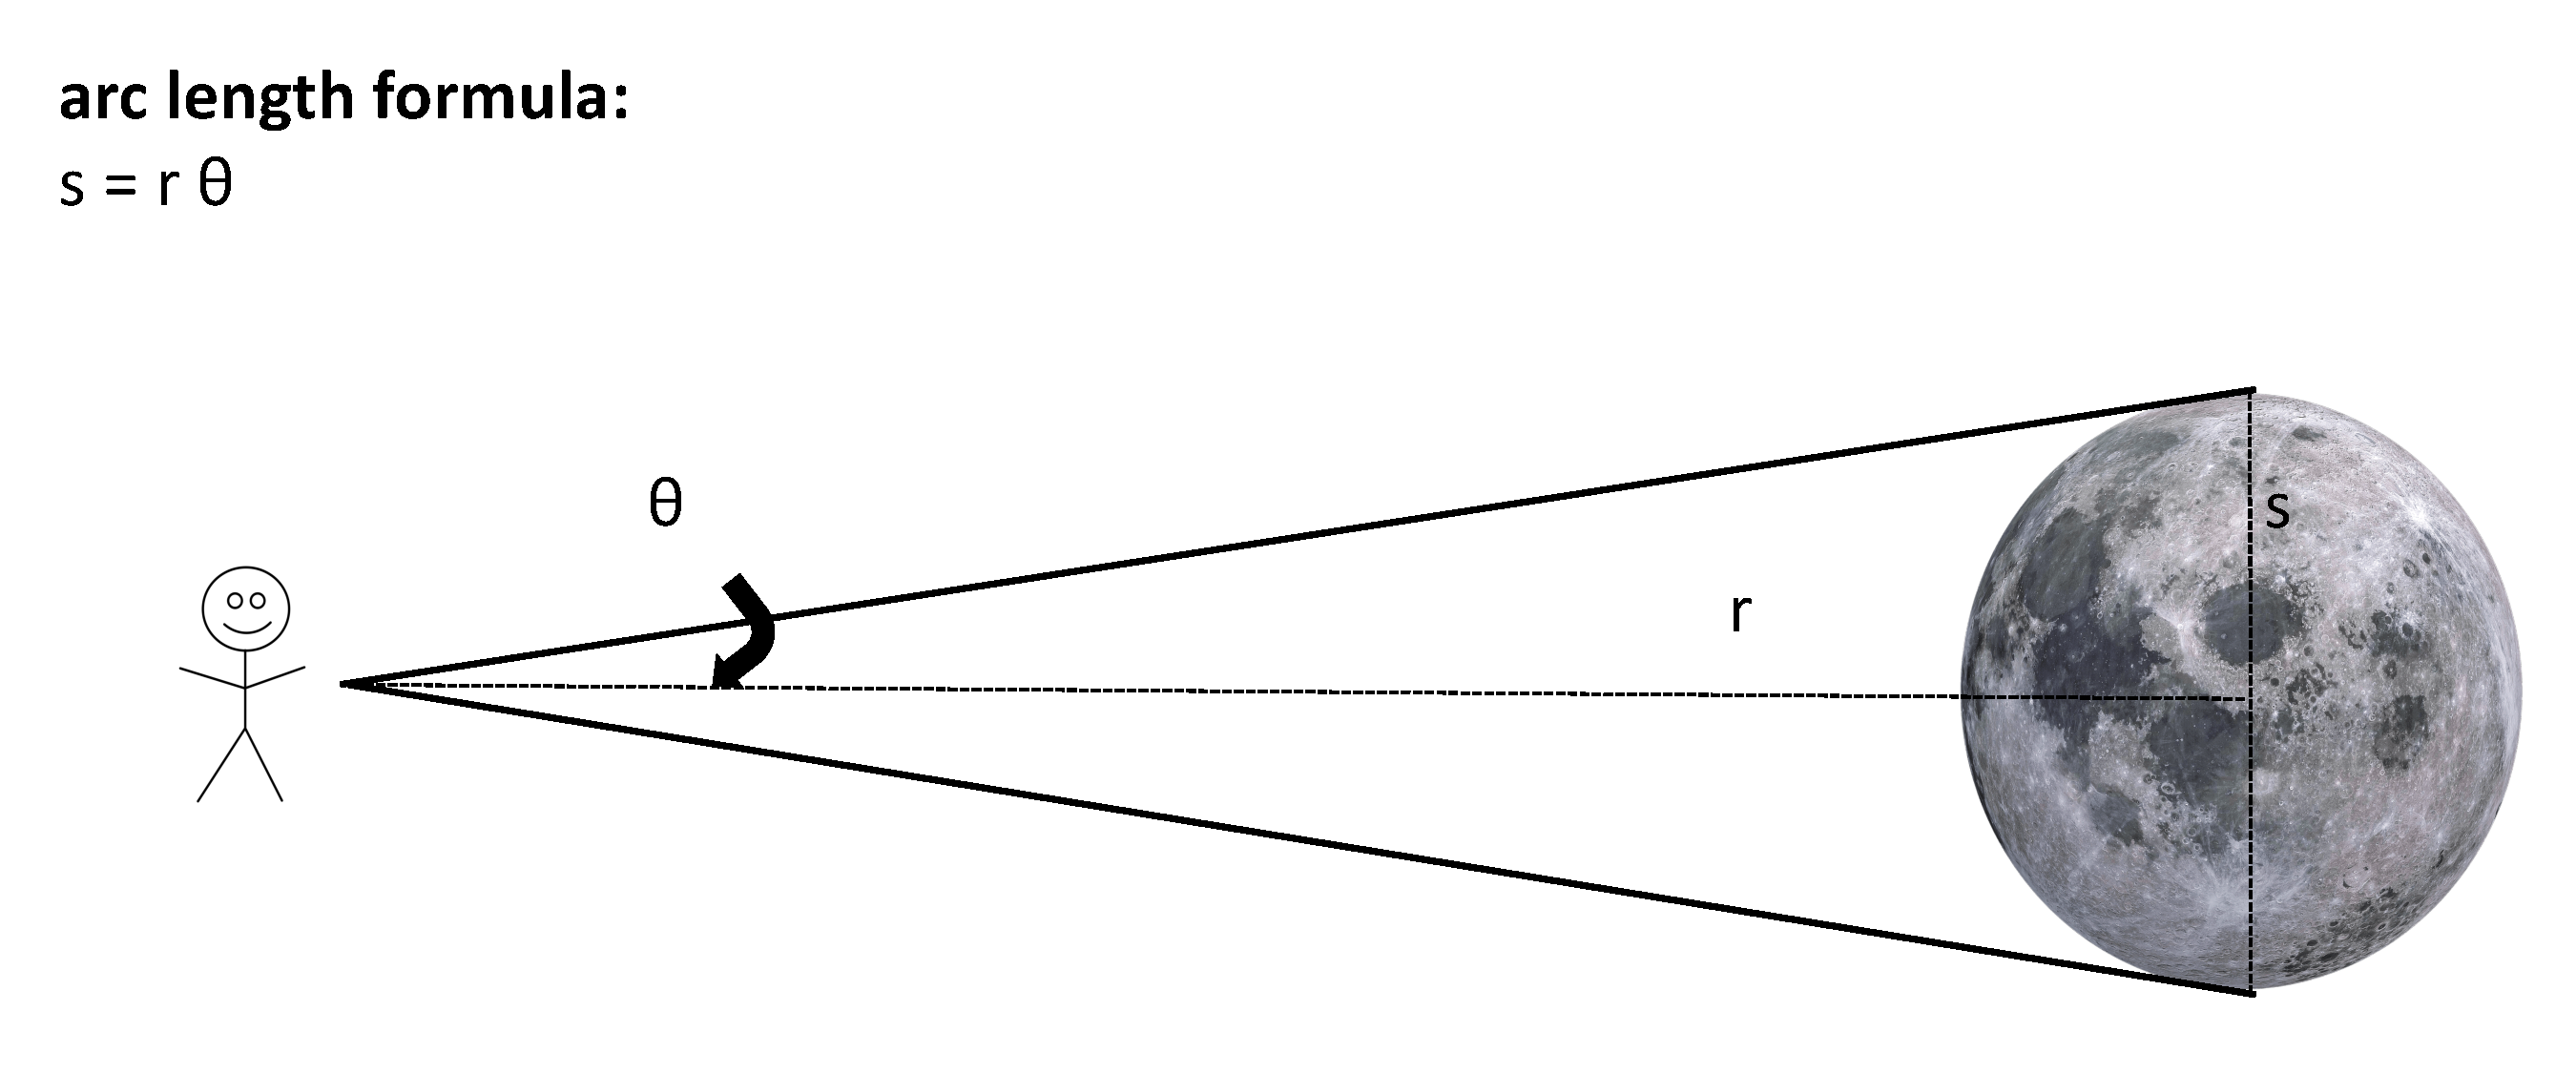
\includegraphics[width=15cm]{arc_length.pdf}
\end{figure}


\begin{enumerate}
    \item What kind of moon was it? (i.e., what phase?)
    Where is the sun? Draw a picture if necessary.
    
    
%If you have a printed copy of your picture from the Moon, use it in the following questions. Otherwise, just use the provided unlabeled photo whenever the lab says to use yours.
    \item Identify and label features on your photo using the provided map.
    
    \item Measure the diameter of some central feature in your photo (avoid features very close to the edge) using a ruler. Use \url{wolframalpha.com} to look up the diameter of that feature and calculate the scale (i.e. the ratio of a distance on the map to the corresponding distance on the Moon surface) of your photo. Your scale should be unitless, so make sure you convert units correctly. 
    
    \item Measure the diameter of the Moon in your photo using a ruler. Based on your scale from the previous question, what is the diameter of the Moon? What is its actual diameter? Was your estimate close? If not, why?
    
    \item We can now use a nifty trick to get an estimate for how for the Moon is from the Earth. We will use the arc length formula, our value for the angular diameter (in radians), and the physical diameter of the Moon to determine the distance to the Moon. In the figure above, s is the diameter of the Moon, r is the distance to the moon, and $\theta$ is the angular diameter of the Moon. Remember you will have to convert your angular diameter from degrees to radians. Using this estimate, how far away is the Moon from the Earth? 
    


%You will print your own photo of the Moon and use it to make some calculations.
%\item Identify the line separating the bright and the dark part (separating line).
%\item Identify the Aristilus crater and the Piton mountain. Measure the distance from the separating line.  Also measure the size of the shadow. We will use some geometry to calculate the depth of the craters and the height of the mountain.
%\item Given that the angular side of the Copernicus crater is 49 arcseconds, calculate the angular size of the Moon. Using this, find the distance of the Moon.
\end{enumerate}


\section{Conclusions}
\begin{enumerate}
    \item The actual mean distance to the Moon is 385,000 km. What is your percent error? What sources of error are there in your measurement?
    % 377369 km at 9pm on October 11, look up using Wolfram Alpha
    
    
    \item As you may have noticed at some point in the past, the Sun and the Moon are about the same angular size on the sky. 
    Use this information, as well as the distance between the Sun and the Earth ($1 \, \mathrm{AU} = 1.5 \e{11} \, \mathrm{m}$), to calculate the radius of the Sun. 
    Compare your answer to the actual solar radius $\mathrm{R}_{\odot} = 7 \e{8} \, \mathrm{m}$.


    \item If the lab was perfectly clear to you, what did you like or dislike? If not, what confused you? Any other feedback?
\end{enumerate}

\end{document}
